\chapter{第五期}

\section{2019年12月2日 星期一 晴}

杨若君

周五我生病了,好了后要休息48小时,所以今天不能上学。到了下午的时候我不知道今天的作业是什么,就在群里问,可是大家都很忙,根本没时间答复。后来好不容易问到了作业,却又不知道是什么意思。最后只好打电话给陈姿伊,我们花了好一会儿才搞清楚。

生病了可真麻烦,以后一定要好好锻炼,保持身体健康。

\section{2019年12月2日 星期一 晴}

余蕙琳

最近妈妈给我买了一双暖拖鞋,拖鞋上面的图案是一串英文字母,其中,字母“D”上面还画着两个小小鹿角。除了字母之外,还有两朵娇嫩的樱花。另一只鞋子上是一只可爱的小鹿。瞧,小鹿的眼晴笑得眯成了一条像月亮一样的弧线,眼睫毛长长的,嘴巴小小的,腮红粉扑扑的。它的两个鹿角向外分叉,而且是立体的。外公看见了这双鞋,对妈妈说:“阿颖,鞋子买错了!”妈妈说:“阿公,设计就是这样设计的。”我听了后哭笑不得,想到了一句话:没文化,真可怕!现在我们一定要努力学习,不要让这句话用到我们身上。

\section{2019年12月2日 星期二 晴}

蒋鲁弋

今天数学小测考了100分,我非常高兴。上完兴趣课就飞快地跑到了校门口。东张西望了会,看到了妈妈,突然心生一计,低下头,默默地走过去。妈妈看到我这个样子就说:“考试不理想,是不是?”我说:“才89分。”妈妈一边走一边说:“是真的吗?……”我在被妈妈骂了几下后说:“才怪,我考了100分!”妈妈急忙拿过书包翻了翻,过了一会,她微笑地说:“不错,有进步,以后继续努力!”我俩坐上车,高高兴兴地回家了。

\section{2019年12月3日 星期二 晴}

戴瑞彤

今天晚上,妈妈给我烧了我最爱的“肉饼蒸蛋”。我看着那鲜红的肉和那黄橙橙的蛋,不禁闻了一下,那香喷喷的气味扑鼻而来。我马上尝了一口,真是色香味浓,回味无穷。我又尝了一口,咦?这是什么味道?我把嘴里的肉饼蒸蛋吐了出来,仔细一看,天哪,这蛋竟然是一些黄色的液体,还没熟呢!看来,看事物不能只看表面,还要看内在。不要被表面给迷惑。

\section{2019年12月3日 星期二 晴}

李恩博

今天科学课下课,周弈儒指着她自己说:“我非肌肉。”我说:“飞鸡肉?什么东西?”“对,非肌肉。”周弈儒说,我听了捧腹大笑。我的笑引来了姚琪,姚琪说:“唉,你笑什么吗?”我一边哈哈大笑一边说:“周弈儒说她飞鸡肉。”姚琪听了也哈哈大笑说:“周弈儒,你停顿不对,是,非——肌肉。”周弈儒说:“对呀,非肌肉。”周弈儒下次要注意停顿。

\section{2019年12月3日 星期二 晴}

施迪文

今天下午,数学成绩出来了。“徐宸诚……,施迪文……”数学老师报道。我的心提到了嗓子眼。听了成绩,我差点一蹦三尺高,我得了满分!

\section{2019年12月5日 星期四 晴}

姚琪

今天中午,语文课上开始做眼保健操时,詹老师说:“姚琪!”我正沉浸在我的专属世界里,突然詹老师的话让我吓了一跳,还以为有什么不好的事呢。于是我赶紧抬起头来,胆战心惊地来到了詹老师面前,原来詹老师是叫我去复印资料。“呼”我松了一口气,赶紧跑到了文印室,由于跑得太急,我没留意地上放着一块板,不小心摔了一跤。哎,这也太尴尬了吧!

\section{2019年12月5日 星期四}

徐诚磊

昨天晚上做完作业,我和妈妈展开了一场惊心动魄的国际象棋对决。我们先各自摆好阵式,开始战斗。我故意声东击西,把她厉害的棋都引到了左边,然后出其不意地把车移到妈妈的王面前,谁知妈妈用“自杀式袭击”把我的车给吃了,我将计就计用兵把吃我车的王后给吃了。妈妈没了王后实力大减,我趁此机会暗度陈仓,趁妈妈不注意,悄无声息地把另一个车移到妈妈的王前,将王了。终于这场对决以我的胜利告一段落。

\section{2019年12月5日 星期四 晴}

孔俞澄

今天我遇到赵奕麟,他拿着一支笔,装扮成一把枪对着我。我说:“你想比枪是吧?”我拿出一个铅笔盒,当成一把大号的枪。他不甘示弱拿出了两本本子当成两把枪。我抓着头皮想该怎么办啊?我拿出一大叠本子当做巨大的枪,他一直想和我比个高下,就拿出书包当做一把巨大大号枪。我搬出一张桌子当做一把巨大巨大号枪,这下他无话可说,很佩服我。

\section{2019年12月9日 星期一 晴}

余蕙琳

今天爸爸带我去吃了日式料理,菜一上,我就开始大吃特吃起来,五颜六色的料理布满吧台,看得我直咽口水。瞧,那儿的寿丝,鱼籽Q弹圆润,肉丝放在鱼籽下面,显得格外有食欲感,最下面的寿丝卷十分美味,黄瓜和胡萝卜,最吸引人的,还是那洒在寿丝上的调料。条料十分丝滑,吃起来不油不腻当当好。当然,还有好多吃的,想要尝尝,那就快快去天街的三味大江户去尝尝那儿的美味吧!

\section{2019年12月11日 星期三 晴}

蒋鲁弋

昨天,我吃完早饭,准备去上学。这时我咳了几下,吐了一口面条。到了学校,我对张思宇说:“离我远一点儿,我今天早上吐了!”他吓得面如土色,马上告诉了老师。老师叫我到校医那里检查,我一边走一边说:“不会真得了病了吧!”到了医务室,医生听了原因,说我可能真的得了病,叫我去医院检查,我吓得惊慌失措。回家后跟妈妈在医院里跑了好几个小时,查出来只是有点感冒,没有啥事。
这可真是个乌龙事件!

\section{2019年12月11日 星期四}

徐诚磊

周末我和夏天祺去星光大道吃饭,突然夏天祺尿急了,要我陪他去厕所。于是我和他一起飞奔向厕所,一到厕所他就一头扎进了里面。这时我抬了一下头,发现上面有一个女生的标志,于是大喊:“夏天琪,快出来!这是女厕所。”他听了急急跑了出来,看看上面的标识,然后红着脸走进了一旁男厕所,我在外面捧腹大笑起来,这真是“慌不择路”啊!

\section{2019年12月11日 星期三 晴}

施迪文

今天体育课上,老师让我们做了一个游戏:将一个排球放在一张大网上,所有人拉住网,将网向上扬,让球弹起来。刚开始,由于我们心不齐,球弹不高。后来我们齐心协力,将网往上用力一扬,球居然飞出了篮球场,落到了车库附近!

\section{2019年12月12日 星期四}

蒋欣恬

今天我正在走路,突然一块石头把我绊倒了,我气急败坏地从地上爬起来,拍了拍腿上的尘土,感受到大腿上有一阵阵痛,拉开裤子一看,发现鲜红的血从伤口中流了出来。我气愤地向石头看去,才发现这里地上的砖被人移高了一点,不仔细看根本发现不了,很容易会摔倒。唉!现在的熊孩子可真多,把快乐建立在别人的痛苦之上,这样真的不好,有人快乐,有人痛苦,何必呢?真倒霉!

\section{2019年12月15日 星期日 晴}

来欣年

今天早上八点半,我们家的“闹钟”又来叫我起床了。我迷糊得睁开眼,一看大吃了一惊,我心想:“真是不看不知道,一看吓一跳啊,八点四十五分了”。我连忙准备好马上出发时,看到了惊人一目:哥哥怎么还在睡觉?我百思不得其解跑到日历旁一看,12月15日竟是星期日,我倒!

\section{2019年12月16日 星期一 晴}

余慧琳

今天下楼梯时,我急急忙忙地跑下来,结果我脚一扭,身子向前倾,重心向左,啪的一声,摔在地上,当我起来时,脚已经扭了。我一瘸一拐地走向餐厅。左脚渐渐地越来越痛,当我吃力地走楼梯时,我已经吃不消了,顿时眼睛红了,鼻子一酸,强忍着不让眼泪流下,当到了位子,捡起分饭手套时,我才在角落里暗暗流泪,但这谁也不知。现在,左脚已经打了石膏,希望他能快快恢复。

\section{2019年12月16日 星期一 晴}

蒋鲁弋

星期六晚上,老爸带着我来到健身房。我看到了许多器材,有跑步机,哑铃,健胸器等等,还有许多我没见过的奇怪器材。我找了个健胸器,把重量调到9千克,我张开双臂,双手紧紧地抓住手柄,然后用尽全力拉向中间,使两个手柄靠拢,我做了一个、两个、三个…… 在我做第十个的时候,我头上已经挂满了一颗颗大大的汗珠,手臂的关节在强烈地疼痛,这个时候我很想放弃,但是我的意志告诉我:“不要放弃,加油,你可以的!”我用尽了九牛二虎之力终于做完了最后一个。我长舒一口气,说:“只要坚持一下,不就可以完成了嘛!”

\section{2019年12月18日 星期三 阴转雨}

姚琪

今天吃晚饭时,我们讨论起新政策——垃圾分类。妈妈说:“现在上海的垃圾分类做得特别好,连人们见面讲的第一句话都特牛!”我连忙追问:“那他们说的是啥?”“说的不是`你好',而是`你是啥个垃圾?”'妈妈说。我想,哎,新政策带给上海的是“你是啥个垃圾”,给杭州带来的会是啥呢?想到这里我便哈哈大笑起来。

\section{2019年12月18日 星期三}

蒋欣恬

今天妈妈对我说:“家里有个好东西等着你哦。”“是什么?”我好奇地问。“到家你就知道了。”妈妈继续保持神秘。一到家我就迫不及待地跑进家里,呀!我的书桌上多了一个招财猫存钱罐,它上面有许多画作,还写着“年年有余”这四个字,妈妈对我说:“妈妈希望你把每一笔零花钱都存起来,所谓积少成多嘛,这样会对你的未来有所帮助。”“好!”我点点头,记下了妈妈说的话。

\section{2019年12月23日 星期一 阴转雨}

丁凝

今天我刚吃完饭,妈妈拿出了一个小蛋糕,那个蛋糕的表面涂着奶油,奶油的上面插着两片小树叶,树叶上有一个蝴蝶结,蝴蝶结上面挂着几个巧克力做的小铃铛和小珠子。奶油的下面有一块蛋糕,蛋糕旁边有一圈草莓,我真想吃这块蛋糕呀!就在这时,妈妈说,我可以吃这块蛋糕。我怕妹妹抢走我的蛋糕,就一下子拿走了,飞也似地跑回房间狼吞虎咽地吃起来,很快,蛋糕就被我吃的只剩下一个塑料底座。

\section{2019年12月26日 星期四 晴}

余蕙琳

今天早上醒来,我一下子坐了起来,伸了个大大的懒腰。正准备穿衣服时,我忽然看见床头柜上放着两袋大大的、红红的东西。仔细凑过去一看,原来是“圣诞老人”送的礼物呀。我赶紧拆开袋子。哇!都是美食哦\ldots,有凯蒂猫图案的曲奇饼干;有南瓜籽夹心的海苔脆;有可爱的字母形饼干;有“全心全意为吃货服务”的公社山楂饼;有纯天然的香蕉片;有Q弹的上海特产——花生牛扎糖;有一只贝亲婴儿的唇膏;还有一套孟建平的期末复习试卷。我数了数,一共有八样礼物呢!而且礼物还包括食品、学习和日用品,非常实在。这次圣诞节真是“收获”满满。

\section{2019年12月26日 星期四 雨}

夏天琪

因为昨天是圣诞节,所以老师为我们准备了好吃的拐杖糖。上面还有一个美丽的装饰糖,有的是一个圣诞拐杖,有的是一个雪人,有的是一棵圣诞树,还有的是一个圣诞老人。他们五颜六色的,样子可爱极了!尝了尝,一股甜丝丝的味道就甜进了我的心房。这就是圣诞节的味道!

\section{后记}

四年级上学期快结束,《闲言碎语》活动进行了快一年的时间,截止目前为止我们已经收录了一共128篇日记。如果打印出来也有厚厚一本呢,这是一个多么了不起的成就!同学们是不是也会惊讶你们怎么能写出那么多文字。难道这不是大家坚持的成果吗?

能有这样的成绩,我想大家首先应该感谢自己,感谢自己即使熬到很晚也要坚持写好当天的日记。大家应该为自己认真对待的态度和坚持到底的毅力感到骄傲。

还要感谢詹老师默默的付出。这本集子收录的日记只有十之一左右,老师每天要花时间为大家的文章点评修改。而且大家目前书写和写作还不是很流畅,读起来会比较吃力。我看过我们组的《闲言碎语》本子,有些文章涂改得惨不忍睹,不过老师还是给圈出错别字,修改病句。老师得有多么强大的心理才能读下去。

前面说到过,练习写作就像练习书法,分为临摹和创作。如果命题作文类似于书法临摹,有一定的格式和套路,那么大家写的闲言碎语就类似于书法创作了。跟书法创作一样,创作写作更能体现一个人的实际水平和内心。格式题材不限,记录自己的所见所思,所以文字是活泼泼的,有温度的。

例如一位同学在日记中写道:“但这件事是我的错,我不该在早读的时间起哄,影响大家早读,希望老师能原谅我,还请您把铁环分给大家。”读到这句话,不由得想到一个带着眼镜胖乎乎的小男孩,有点调皮,更有一颗善良乐意分享的心,老师读了估计火气也没了吧。

2020年再接再厉!

\begin{figure}[htb]
    \centering
    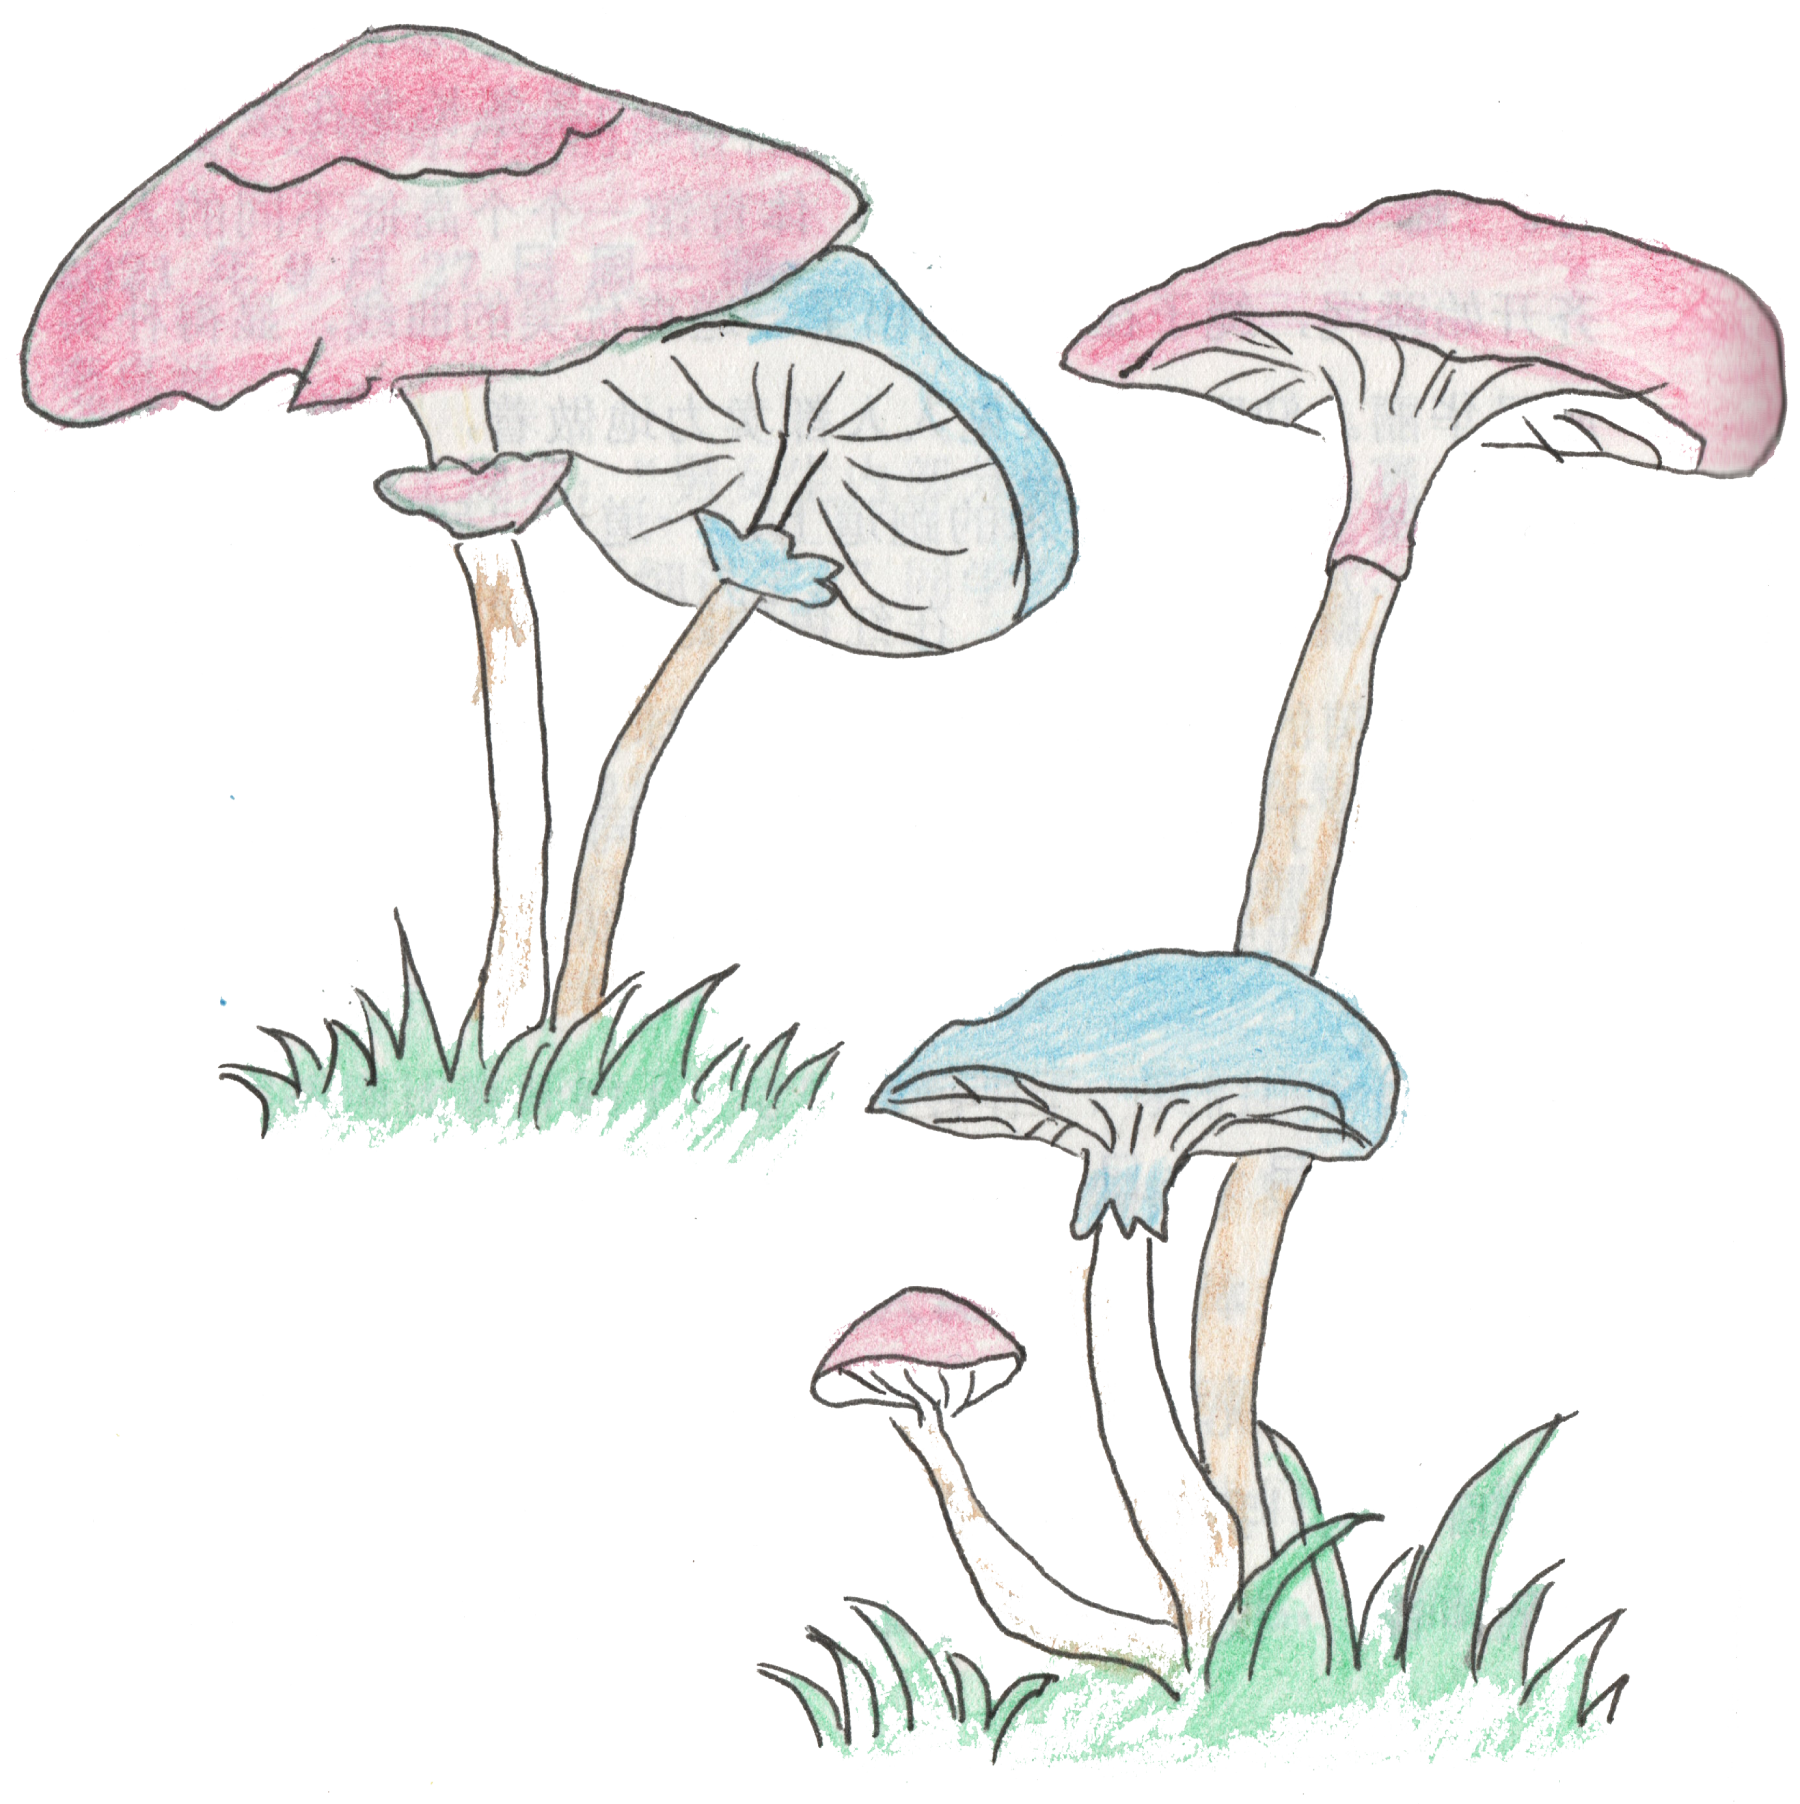
\includegraphics[width=0.8\textwidth]{figure/05.png}
\end{figure}